% Native TikZ figure 1.50; geometry measured from reference PDF page 83.
% Ground-left source coordinate (408.495,678.173) bp, y upwards here.
\newcommand{\ReplicaGravityDiagram}{%
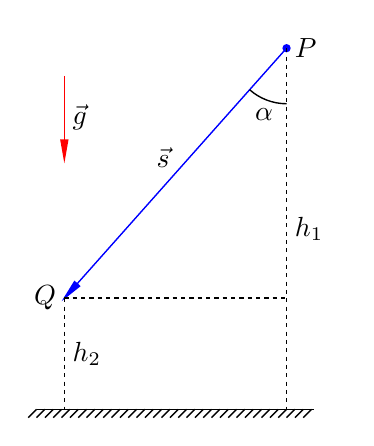
\begin{tikzpicture}[x=1bp,y=1bp,line width=.5bp,
 every node/.style={inner sep=0pt,outer sep=0pt,font=\fontsize{10}{12}\selectfont}]
  \coordinate (P) at (90,130);
  \coordinate (Q) at (10,40);
  \draw (0,0)--(100,0);
  \foreach \x in {0,3,...,99} {\draw (\x,0)--++(-3,-3);}
  \fill[blue] (P) circle[radius=1.5bp];
  \draw[blue] (P)--(Q);
  \filldraw[blue] (13.67166,45.96033)--(Q)--(15.48874,44.34509)--cycle;
  \draw[dash pattern=on 1.5bp off 1.5bp] (P)--(90,0);
  \draw[dash pattern=on 1.5bp off 1.5bp] (Q)--(10,0);
  \draw[dash pattern=on 1.5bp off 1.5bp] (Q)--(90,40);
  \node[anchor=base west] at (93,126.596) {$P$};
  \node[anchor=base west] at (-.876,37.564) {$Q$};
  \node[anchor=base west] at (43.2296,87.100) {$\vec s$};
  \node[anchor=base west] at (93,62.287) {$h_1$};
  \node[anchor=base west] at (13,17.287) {$h_2$};
  \draw (90,110) arc[start angle=270,end angle=228.37,radius=20];
  \node[anchor=base west] at (78.687,104.016) {$\alpha$};
  \draw[red] (10,120)--(10,90);
  \filldraw[red] (8.7845,96.89374)--(10,90)--(11.2155,96.89374)--cycle;
  \node[anchor=base west] at (13.00238,102.409) {$\vec g$};
  % Preserve the old macro's TeX box and baseline, so text flow stays fixed.
  \pgfresetboundingbox
  \pgfpathrectangle{\pgfpoint{-3.2bp}{-3.2bp}}{\pgfpoint{114.85211pt}{141.11418pt}}
  \pgfusepath{use as bounding box}
\end{tikzpicture}%
}
